\section{Causas raíz}
    \label{fig:causas}
El incidente comenzó con una interrupción de conectividad de 43 segundos \cite{Warner2018}
entre dos instalaciones de GitHub en la costa este de Estados Unidos. Esta desconexión momentánea provocó 
que Orchestrator promoviera réplicas de MySQL ubicadas en la costa oeste, aunque todavía existían escrituras que estaban 
pendientes de replicación, lo cual dio como resultado que las bases de datos quedaran en estados diferentes entre ambas regiones \cite{Warner2018}.
La recuperación fue complicada porque la nueva topología de MySQL no era compatible y generaba latencia entre regiones. Además, fue necesario restaurar respaldos, sincronizar réplicas y procesar trabajos acumulados. 
Estas condiciones prolongaron la degradación del servicio \cite{Warner2018}.
\begin{figure}[H]
    \centering
    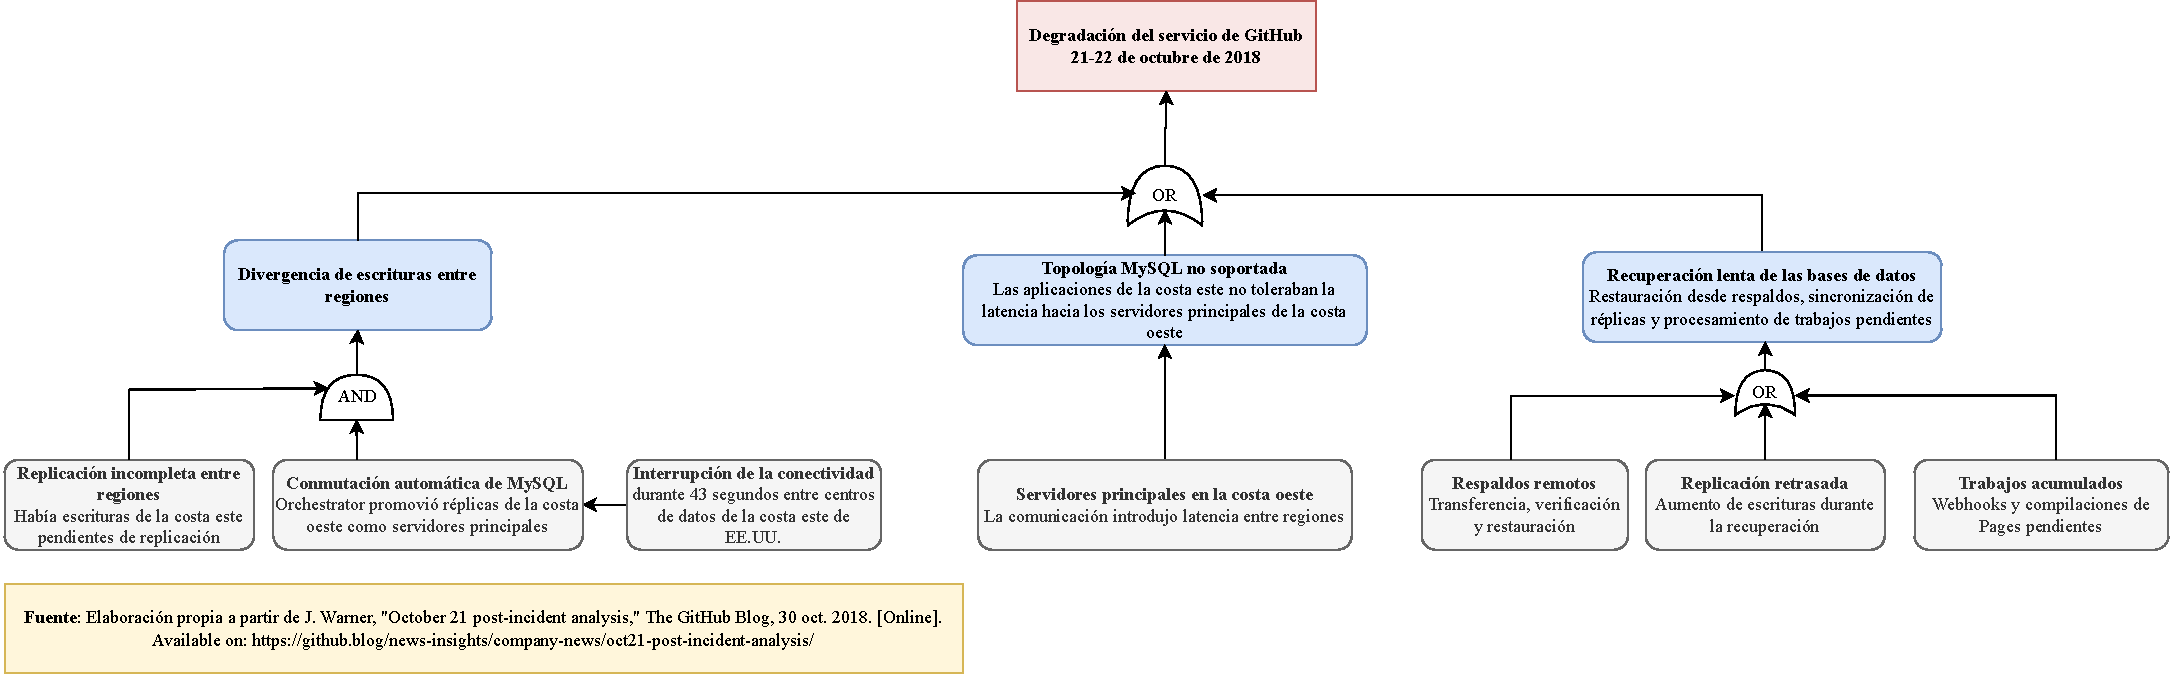
\includegraphics[width=\textwidth]{causas.pdf}
    \caption{Árbol de fallos del incidente de GitHub de octubre de 2018. Elaboración propia a partir de \cite{Warner2018}.}
\end{figure}